\begin{figure}

  \setlength{\unitlength}{\textwidth}
  \begin{picture}(1,0.75)(0,0.35)
    
    % % %90
      \put(0,0.9){\includegraphics[width=0.35\unitlength]{../FnP/gnuplot/power_time_history_90.eps}}
      \put(0,.68){\includegraphics[width=0.35\unitlength]{../FnP/gnuplot/f_y_history_90.eps}}
      \put(0,0.46){\includegraphics[width=0.35\unitlength]{../FnP/gnuplot/theta_time_history_90.eps}}
      
      % %165
       \put(0.33,0.9){\includegraphics[width=0.35\unitlength]{../FnP/gnuplot/power_time_history_165.eps}}
       \put(0.33,.68){\includegraphics[width=0.35\unitlength]{../FnP/gnuplot/f_y_history_165.eps}}
       \put(0.33,0.46){\includegraphics[width=0.35\unitlength]{../FnP/gnuplot/theta_time_history_165.eps}}
       
       \put(0.65,0.9){\includegraphics[width=0.35\unitlength]{../FnP/gnuplot/power_time_history_400.eps}}
       \put(0.65,.68){\includegraphics[width=0.35\unitlength]{../FnP/gnuplot/f_y_history_400.eps}}
       \put(0.65,0.46){\includegraphics[width=0.35\unitlength]{../FnP/gnuplot/theta_time_history_400.eps}}
      
            
      
      
   
 	\put(0.5,0.43){\large $\frac{tU}{D}$}
 	\put(0.15,0.43){\large $\frac{tU}{D}$}
    \put(0.8,0.43){\large $\frac{tU}{D}$}
    
   
   	
   	\put(-0.04,1.0){$\frac{P}{\rho \mathcal{A}U^3}$}
    \put(-0.02,0.75){$F_y$}
    \put(-0.02,0.55){$\theta$}
   	

    \put(0.05,0.88){(a)}
    \put(0.05,0.66){(d)}
    \put(0.05,0.43){(g)}
    
    \put(0.38,0.88){(b)}
    \put(0.38,0.66){(e)}
    \put(0.38,0.43){(h)}
    
    \put(0.68,0.88){(c)}
    \put(0.68,0.66){(f)}
    \put(0.68,0.43){(i)}
       

  \end{picture}

  \caption{Time histories of $P_t$,$P_d$,$F_y$ and $\theta$ at $\ustar=90,165$ and $400$ where the mean power dissipated due to mechanical was calculated using equation \hilight{equation}. Data was obtained at $\zeta=0.1$ and $m^*=40$. The time histories of $P_t$ ( \solidrule[4mm]\hspace{1mm}) and $P_d$ (\protect\dashedrule) are presented in (a), (b) and (c) where \ustar is 90, 165 and 400 respectively.(d), (e) and (f) shows time histories of the instantaneous force $F_y$ and (g), (h) and (i) shows the time history of the instantaneous angle $\theta$ of the corresponding power plots above}
    \label{fig:power_time_histories}
\end{figure}




